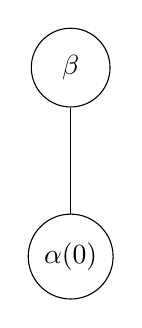
\begin{tikzpicture}[yscale=1.2,every node/.style={circle,draw,minimum size = 10 mm}]
  \node (b) at (1,0) {$\beta$};
    \node (a) at (1,-2) {$\alpha(0)$};
    \draw (b) -- (a);
\end{tikzpicture}
\quad
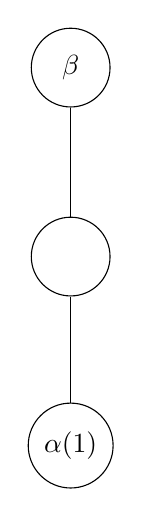
\begin{tikzpicture}[yscale=1.2,every node/.style={circle,draw,minimum size = 10 mm}]
  \node (b) at (1,0) {$\beta$};
  \node (c) at (1, -2) {};
    \node (a) at (1,-4) {$\alpha(1)$};
    \draw (c) -- (a);
    \draw (b) -- (c);
\end{tikzpicture}